\begin{frame}
  \frametitle{Open development}
  What is it?
  
  {\it Hint}: distinct from {\it open-source} development
  \pause\medskip

  An answer:

  The combination of develpoment practices that emphasizes reproducibility at all scales of the development cycle:
  \begin{itemize}
      \item individual commits
      \item designing bug fixes and features
  \end{itemize}
\end{frame}
    

\begin{frame}[fragile]
    \frametitle{Open development example}
    \framesubtitle{Implementing OpenMC in SaltProc}

    Idea: Implement OpenMC in an open-source Molten Salt Reactor depletion simulator 
    \newline
    \newline
    In the issue tracker, I detail background/motivation and the description of the idea:


    \vspace{0.5cm}
    \begin{figure}[htpb]
        \centering
        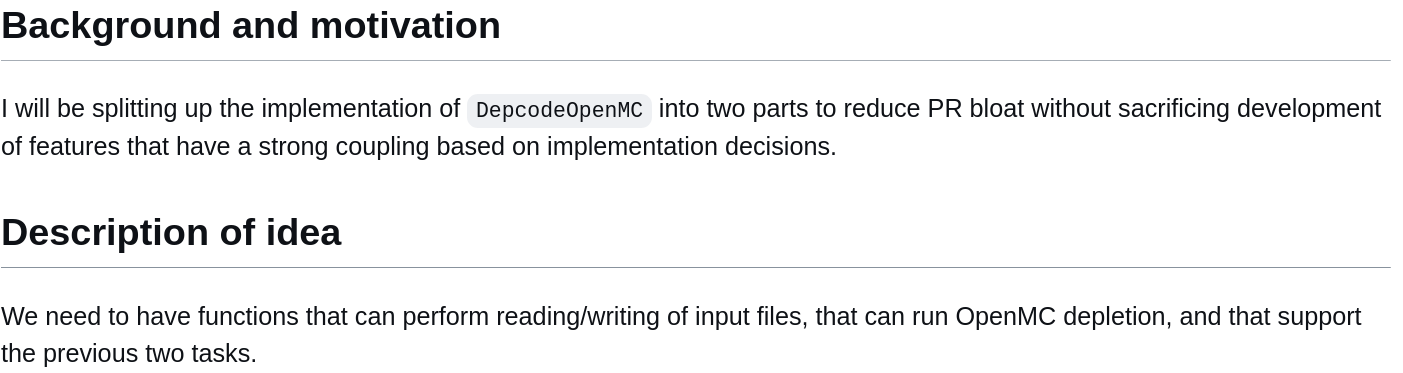
\includegraphics[width=10cm]{images/open-dev-ex1.png}
    \end{figure}

    
\end{frame}

\begin{frame}[fragile]
    \frametitle{Open development example}
    \framesubtitle{Implementing OpenMC in SaltProc}

    I also detail a skeleton design/implementation:


    \vspace{0.5cm}
    \begin{figure}[htpb]
        \centering
        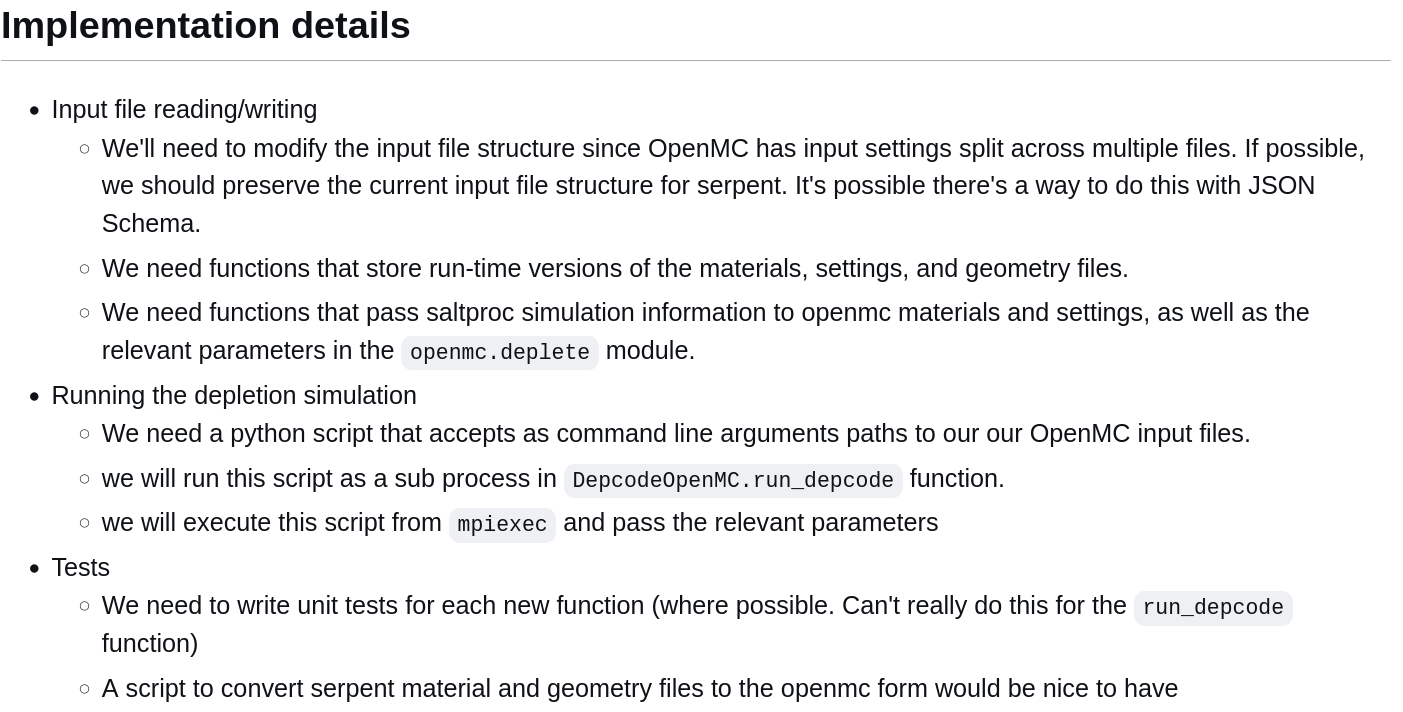
\includegraphics[width=10cm]{images/open-dev-ex2.png}
    \end{figure}

\end{frame}

\begin{frame}[fragile]
    \frametitle{Open development example}
    \framesubtitle{Implementing OpenMC in SaltProc}

    Finally, I write down any snags I can think of:
    \vspace{0.5cm}
    \begin{figure}[htpb]
        \centering
        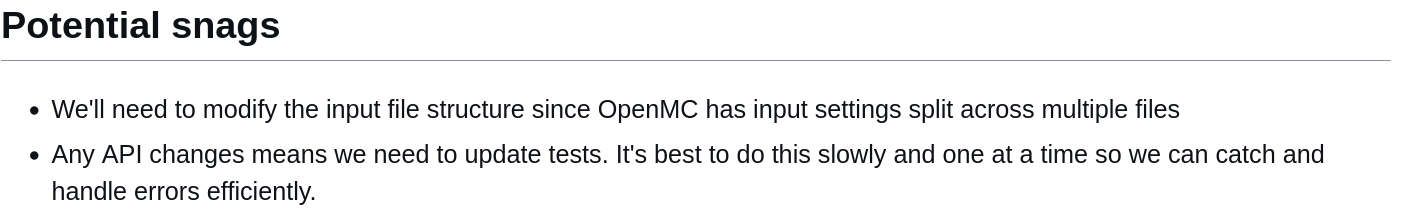
\includegraphics[width=10cm]{images/open-dev-ex3.png}
    \end{figure}

\end{frame}
